\documentclass[tikz,border=5pt]{standalone}
\usepackage[utf8]{inputenc}
\usepackage[T1]{fontenc}
\usepackage{amssymb}
\usetikzlibrary{shapes,arrows.meta,positioning,calc,decorations.markings,patterns}

\begin{document}
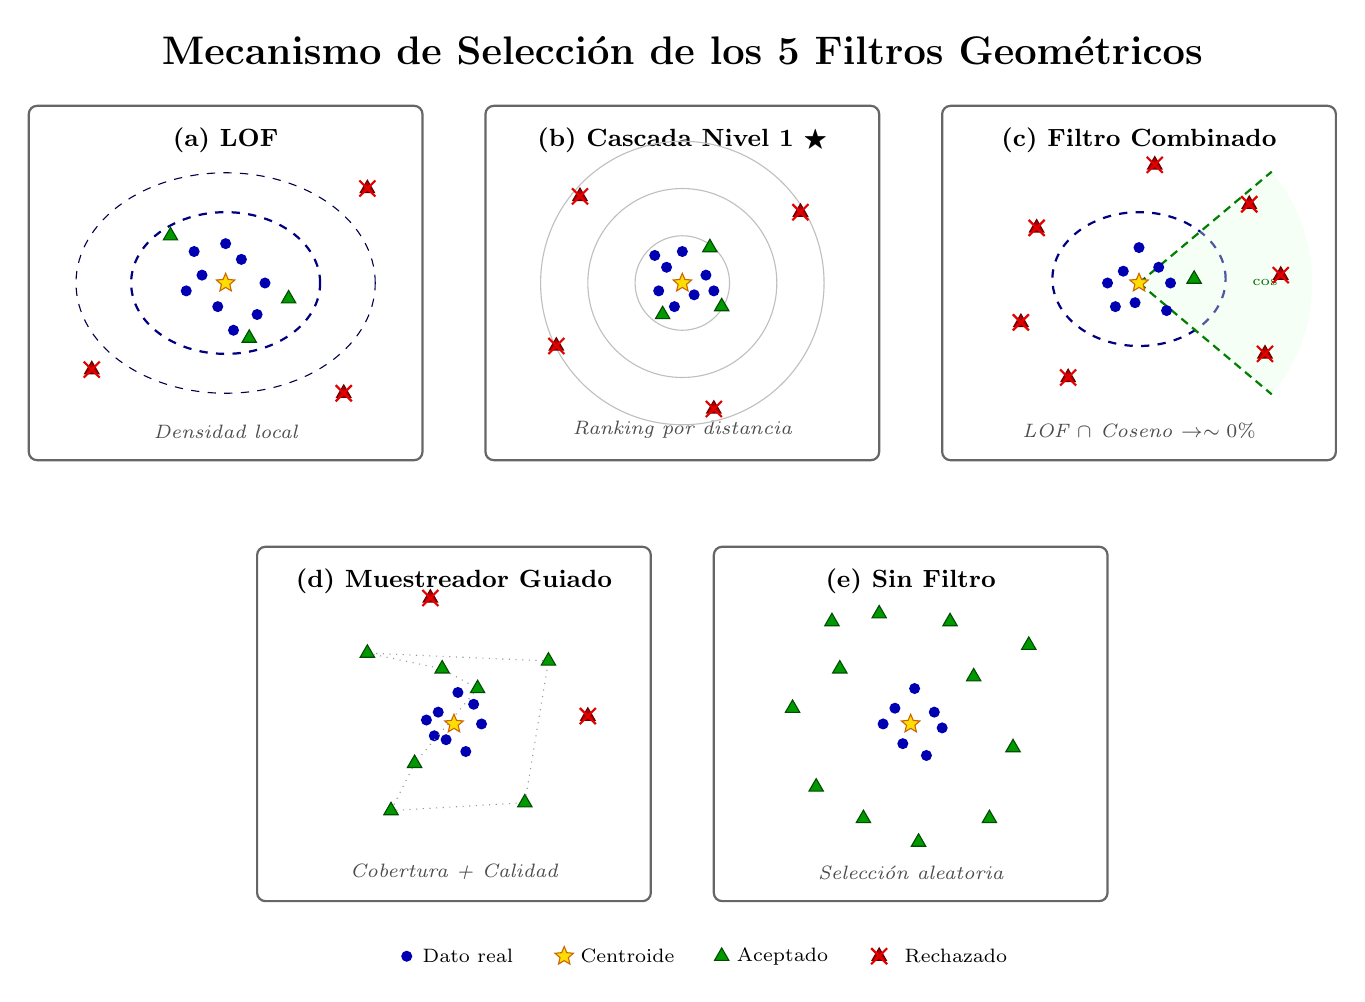
\begin{tikzpicture}[
    % --- common styles ---
    real point/.style={circle, fill=blue!70!black, inner sep=0pt, minimum size=4pt},
    centroid/.style={star, star points=5, star point ratio=2.2, fill=yellow!80!orange,
                     draw=orange!80!black, inner sep=0pt, minimum size=7pt},
    accepted/.style={regular polygon, regular polygon sides=3, fill=green!60!black,
                     draw=green!30!black, inner sep=0pt, minimum size=6pt},
    rejected/.style={regular polygon, regular polygon sides=3, fill=red!70!black,
                     draw=red!40!black, inner sep=0pt, minimum size=6pt},
    cross mark/.style={cross out, draw=red!90!black, thick, minimum size=5pt, inner sep=0pt},
    panel/.style={draw=black!60, thick, rounded corners=3pt, fill=white},
    panel title/.style={font=\bfseries\small, anchor=north},
    panel label/.style={font=\scriptsize\itshape, text=black!70, anchor=south},
]

% =============================================================
%  Layout constants
% =============================================================
\def\pw{5.0}   % panel width
\def\ph{4.5}   % panel height
\def\gx{5.8}   % horizontal gap (center to center)
\def\gy{5.6}   % vertical gap (center to center)

% =============================================================
%  Main title
% =============================================================
\node[font=\Large\bfseries, anchor=south] at (1*\gx, 0.5*\ph+0.4)
    {Mecanismo de Selecci\'{o}n de los 5 Filtros Geom\'{e}tricos};

% =============================================================
%  PANEL (a)  --  LOF
% =============================================================
\begin{scope}[shift={(0,0)}]
  % frame
  \draw[panel] (-0.5*\pw,-0.5*\ph) rectangle (0.5*\pw,0.5*\ph);
  \node[panel title] at (0,0.5*\ph-0.15) {(a) LOF};
  \node[panel label] at (0,-0.5*\ph+0.15) {Densidad local};

  % real data cluster
  \node[real point] (a1) at (-0.3, 0.1) {};
  \node[real point] (a2) at ( 0.2, 0.3) {};
  \node[real point] (a3) at (-0.1,-0.3) {};
  \node[real point] (a4) at ( 0.5, 0.0) {};
  \node[real point] (a5) at ( 0.0, 0.5) {};
  \node[real point] (a6) at ( 0.4,-0.4) {};
  \node[real point] (a7) at (-0.5,-0.1) {};
  \node[real point] (a8) at ( 0.1,-0.6) {};
  \node[real point] (a9) at (-0.4, 0.4) {};

  % centroid
  \node[centroid] at (0.0, 0.0) {};

  % density contours (dashed irregular ellipses)
  \draw[dashed, blue!50!black, thick]
    (0.0,0.0) ellipse (1.2 and 0.9);
  \draw[dashed, blue!30!black]
    (0.0,0.0) ellipse (1.9 and 1.4);

  % accepted (inside contours)
  \node[accepted] at (-0.7, 0.6) {};
  \node[accepted] at ( 0.8,-0.2) {};
  \node[accepted] at ( 0.3,-0.7) {};

  % rejected (outside contours)
  \node[rejected] at ( 1.8, 1.2) {};
  \node[cross mark] at ( 1.8, 1.2) {};
  \node[rejected] at (-1.7,-1.1) {};
  \node[cross mark] at (-1.7,-1.1) {};
  \node[rejected] at ( 1.5,-1.4) {};
  \node[cross mark] at ( 1.5,-1.4) {};
\end{scope}

% =============================================================
%  PANEL (b)  --  Cascada Nivel 1
% =============================================================
\begin{scope}[shift={(\gx,0)}]
  \draw[panel] (-0.5*\pw,-0.5*\ph) rectangle (0.5*\pw,0.5*\ph);
  \node[panel title] at (0,0.5*\ph-0.15) {(b) Cascada Nivel 1 $\bigstar$};
  \node[panel label] at (0,-0.5*\ph+0.15) {Ranking por distancia};

  % concentric distance rings
  \draw[gray!50, thin]  (0,0) circle (0.6);
  \draw[gray!50, thin]  (0,0) circle (1.2);
  \draw[gray!50, thin]  (0,0) circle (1.8);

  % real data
  \node[real point] at (-0.2, 0.2) {};
  \node[real point] at ( 0.3, 0.1) {};
  \node[real point] at (-0.1,-0.3) {};
  \node[real point] at ( 0.4,-0.1) {};
  \node[real point] at ( 0.0, 0.4) {};
  \node[real point] at (-0.3,-0.1) {};
  \node[real point] at ( 0.15,-0.15) {};
  \node[real point] at (-0.35, 0.35) {};

  % centroid
  \node[centroid] at (0,0) {};

  % accepted (close)
  \node[accepted] at ( 0.35, 0.45) {};
  \node[accepted] at (-0.25,-0.4) {};
  \node[accepted] at ( 0.5, -0.3) {};

  % rejected (far)
  \node[rejected] at ( 1.5, 0.9) {};
  \node[cross mark] at ( 1.5, 0.9) {};
  \node[rejected] at (-1.3, 1.1) {};
  \node[cross mark] at (-1.3, 1.1) {};
  \node[rejected] at ( 0.4,-1.6) {};
  \node[cross mark] at ( 0.4,-1.6) {};
  \node[rejected] at (-1.6,-0.8) {};
  \node[cross mark] at (-1.6,-0.8) {};
\end{scope}

% =============================================================
%  PANEL (c)  --  Filtro Combinado
% =============================================================
\begin{scope}[shift={(2*\gx,0)}]
  \draw[panel] (-0.5*\pw,-0.5*\ph) rectangle (0.5*\pw,0.5*\ph);
  \node[panel title] at (0,0.5*\ph-0.15) {(c) Filtro Combinado};
  \node[panel label] at (0,-0.5*\ph+0.15) {LOF $\cap$ Coseno $\rightarrow \sim 0\%$};

  % density contour
  \draw[dashed, blue!50!black, thick]
    (0.0,0.05) ellipse (1.1 and 0.85);

  % angular / cosine threshold region (wedge)
  \fill[green!10!white, opacity=0.35]
    (0,0) -- (40:2.2) arc (40:-40:2.2) -- cycle;
  \draw[green!50!black, thick, densely dashed]
    (0,0) -- (40:2.2);
  \draw[green!50!black, thick, densely dashed]
    (0,0) -- (-40:2.2);
  \node[font=\tiny, green!40!black] at (1.6,0) {cos};

  % real data
  \node[real point] at (-0.2, 0.15) {};
  \node[real point] at ( 0.25, 0.2) {};
  \node[real point] at (-0.05,-0.25) {};
  \node[real point] at ( 0.4, 0.0) {};
  \node[real point] at ( 0.0, 0.45) {};
  \node[real point] at ( 0.35,-0.35) {};
  \node[real point] at (-0.4, 0.0) {};
  \node[real point] at (-0.3,-0.3) {};

  % centroid
  \node[centroid] at (0,0) {};

  % only one barely accepted (intersection is tiny)
  \node[accepted] at (0.7, 0.05) {};

  % everything else rejected
  \node[rejected] at ( 1.4, 1.0) {};
  \node[cross mark] at ( 1.4, 1.0) {};
  \node[rejected] at (-1.3, 0.7) {};
  \node[cross mark] at (-1.3, 0.7) {};
  \node[rejected] at ( 1.6,-0.9) {};
  \node[cross mark] at ( 1.6,-0.9) {};
  \node[rejected] at (-0.9,-1.2) {};
  \node[cross mark] at (-0.9,-1.2) {};
  \node[rejected] at ( 0.2, 1.5) {};
  \node[cross mark] at ( 0.2, 1.5) {};
  \node[rejected] at (-1.5,-0.5) {};
  \node[cross mark] at (-1.5,-0.5) {};
  \node[rejected] at ( 1.8, 0.1) {};
  \node[cross mark] at ( 1.8, 0.1) {};
\end{scope}

% =============================================================
%  PANEL (d)  --  Muestreador Guiado
% =============================================================
\begin{scope}[shift={(0.5*\gx,-\gy)}]
  \draw[panel] (-0.5*\pw,-0.5*\ph) rectangle (0.5*\pw,0.5*\ph);
  \node[panel title] at (0,0.5*\ph-0.15) {(d) Muestreador Guiado};
  \node[panel label] at (0,-0.5*\ph+0.15) {Cobertura + Calidad};

  % real data
  \node[real point] at (-0.2, 0.15) {};
  \node[real point] at ( 0.25, 0.25) {};
  \node[real point] at (-0.1,-0.2) {};
  \node[real point] at ( 0.35, 0.0) {};
  \node[real point] at ( 0.05, 0.4) {};
  \node[real point] at (-0.35, 0.05) {};
  \node[real point] at ( 0.15,-0.35) {};
  \node[real point] at (-0.25,-0.15) {};

  % centroid
  \node[centroid] (dc) at (0,0) {};

  % selected samples: mix of near centroid (quality) and edges (coverage)
  \node[accepted] (ds1) at ( 0.3, 0.45) {};
  \node[accepted] (ds2) at (-0.5,-0.5) {};
  \node[accepted] (ds3) at ( 1.2, 0.8) {};
  \node[accepted] (ds4) at (-1.1, 0.9) {};
  \node[accepted] (ds5) at ( 0.9,-1.0) {};
  \node[accepted] (ds6) at (-0.8,-1.1) {};
  \node[accepted] (ds7) at (-0.15, 0.7) {};

  % dotted lines showing spread / diversity connections
  \draw[dotted, black!40, thin] (ds1) -- (ds2);
  \draw[dotted, black!40, thin] (ds2) -- (ds6);
  \draw[dotted, black!40, thin] (ds6) -- (ds5);
  \draw[dotted, black!40, thin] (ds5) -- (ds3);
  \draw[dotted, black!40, thin] (ds3) -- (ds4);
  \draw[dotted, black!40, thin] (ds4) -- (ds7);
  \draw[dotted, black!40, thin] (ds7) -- (ds1);

  % rejected (a few, for contrast)
  \node[rejected] at ( 1.7, 0.1) {};
  \node[cross mark] at ( 1.7, 0.1) {};
  \node[rejected] at (-0.3, 1.6) {};
  \node[cross mark] at (-0.3, 1.6) {};
\end{scope}

% =============================================================
%  PANEL (e)  --  Sin Filtro
% =============================================================
\begin{scope}[shift={(1.5*\gx,-\gy)}]
  \draw[panel] (-0.5*\pw,-0.5*\ph) rectangle (0.5*\pw,0.5*\ph);
  \node[panel title] at (0,0.5*\ph-0.15) {(e) Sin Filtro};
  \node[panel label] at (0,-0.5*\ph+0.15) {Selecci\'{o}n aleatoria};

  % real data
  \node[real point] at (-0.2, 0.2) {};
  \node[real point] at ( 0.3, 0.15) {};
  \node[real point] at (-0.1,-0.25) {};
  \node[real point] at ( 0.4,-0.05) {};
  \node[real point] at ( 0.05, 0.45) {};
  \node[real point] at (-0.35, 0.0) {};
  \node[real point] at ( 0.2,-0.4) {};

  % centroid
  \node[centroid] at (0,0) {};

  % all candidates accepted (neutral -- all green, spread everywhere)
  \node[accepted] at ( 0.8, 0.6) {};
  \node[accepted] at (-0.9, 0.7) {};
  \node[accepted] at ( 1.3,-0.3) {};
  \node[accepted] at (-1.2,-0.8) {};
  \node[accepted] at ( 0.5, 1.3) {};
  \node[accepted] at (-0.6,-1.2) {};
  \node[accepted] at ( 1.5, 1.0) {};
  \node[accepted] at (-1.5, 0.2) {};
  \node[accepted] at ( 0.1,-1.5) {};
  \node[accepted] at (-0.4, 1.4) {};
  \node[accepted] at ( 1.0,-1.2) {};
  \node[accepted] at (-1.0, 1.3) {};
\end{scope}

% =============================================================
%  Legend (below panels)
% =============================================================
\begin{scope}[shift={(1*\gx, -\gy - 0.5*\ph - 0.7)}]
  \node[real point, label={[font=\scriptsize]right:Dato real}] at (-3.5, 0) {};
  \node[centroid, label={[font=\scriptsize]right:Centroide}] at (-1.5, 0) {};
  \node[accepted, label={[font=\scriptsize]right:Aceptado}] at (0.5, 0) {};
  \node[rejected] at (2.5, 0) {};
  \node[cross mark] at (2.5, 0) {};
  \node[font=\scriptsize, anchor=west] at (2.7, 0) {Rechazado};
\end{scope}

\end{tikzpicture}
\end{document}
